\documentclass[aspectratio=169,10pt]{beamer}

% --- Engine-Aware Clean Modern Fonts (Inter + JetBrains Mono in XeLaTeX/Tectonic; FiraSans in pdfLaTeX) ---
\usepackage{iftex}
\ifPDFTeX
  \usepackage[T1]{fontenc}
  \usepackage[sfdefault]{FiraSans}
  \usepackage[scale=0.86]{FiraMono}
\else
  \usepackage{fontspec}
  \setsansfont{Inter}[
    UprightFont = *,
    BoldFont = * Bold,
    ItalicFont = * Italic,
    BoldItalicFont = * Bold Italic
  ]
  \setmonofont{JetBrains Mono}[Scale=0.84]
  \renewcommand{\familydefault}{\sfdefault}
\fi

% --- Packages ---
\usepackage{amssymb}
\usepackage{graphicx}
\usepackage{booktabs}
\usepackage{array}
\usepackage{xcolor}
\usepackage{tikz}
\usetikzlibrary{positioning,arrows.meta,fit,backgrounds,calc}
\usepackage{pgfplots}
\pgfplotsset{compat=1.18}
\usepackage{xurl}
\usepackage{hyperref}

% --- Strict Two-Tone Academic Palette (Slate Navy + Restrained Crimson) ---
\definecolor{ink}{HTML}{0F172A}
\definecolor{slate}{HTML}{475569}
\definecolor{muted}{HTML}{64748B}
\definecolor{rulegray}{HTML}{CBD5E1}
\definecolor{tint}{HTML}{F8FAFC}
\definecolor{accent}{HTML}{B91C1C}
\definecolor{okgreen}{HTML}{15803D}

% --- Pure Minimalist Academic Beamer Theme (No boxes, no shadows, no gradients) ---
\usetheme{default}
\setbeamertemplate{navigation symbols}{}
\setbeamersize{text margin left=0.85cm, text margin right=0.85cm}

\setbeamercolor{normal text}{fg=ink, bg=white}
\setbeamercolor{structure}{fg=ink}
\setbeamercolor{frametitle}{fg=ink, bg=white}
\setbeamercolor{itemize item}{fg=accent}
\setbeamercolor{itemize subitem}{fg=slate}
\setbeamercolor{enumerate item}{fg=accent}
\setbeamertemplate{itemize item}{\raisebox{0.18ex}{\tiny\rule{3.2pt}{3.2pt}}}
\setbeamertemplate{itemize subitem}{\scriptsize--}

% --- Clean Frametitle with Hairline Rule ---
\setbeamertemplate{frametitle}{%
  \vspace*{0.22cm}%
  \begin{beamercolorbox}[wd=\textwidth,leftskip=0pt,rightskip=0pt]{frametitle}%
    {\large\bfseries\color{ink}\insertframetitle}%
  \end{beamercolorbox}%
  \vspace{3pt}%
  {\color{rulegray}\hrule height 0.6pt}%
  \vspace{4pt}%
}

% --- Minimal Footer (Subtle hairlines + slide number) ---
\setbeamertemplate{footline}{%
  \ifnum\value{framenumber}>1
  \begin{tikzpicture}[remember picture,overlay]
    \draw[rulegray, line width=0.4pt] ([xshift=0.85cm, yshift=16pt]current page.south west) -- ([xshift=-0.85cm, yshift=16pt]current page.south east);
    \pgfmathsetmacro{\progress}{\insertframenumber/\inserttotalframenumber}
    \draw[accent, line width=1.1pt] ([xshift=0.85cm, yshift=16pt]current page.south west) -- ++(\progress*\textwidth, 0);
    \node[anchor=west, font=\fontsize{6.6}{7.6}\selectfont, text=muted] at ([xshift=0.85cm, yshift=8.5pt]current page.south west)
      {SurakshaNet \;\textbar\; Department of CSE, IIT Ropar};
    \node[anchor=east, font=\fontsize{6.6}{7.6}\selectfont, text=muted] at ([xshift=-0.85cm, yshift=8.5pt]current page.south east)
      {\textbf{\color{ink}\insertframenumber} / \inserttotalframenumber};
  \end{tikzpicture}%
  \vspace*{19pt}%
  \fi
}

% --- Crisp Hairline Frame Helper for Real Screenshots ---
\setlength{\fboxsep}{0pt}
\setlength{\fboxrule}{0.5pt}
\newcommand{\shot}[2]{%
  \fcolorbox{rulegray}{white}{\includegraphics[#1]{#2}}%
}

% --- Minimalist Rectilinear TikZ Styles ---
\tikzset{
  sysbox/.style={draw=ink!75, fill=tint, line width=0.6pt, align=center, font=\fontsize{6.8}{8.2}\selectfont, inner sep=4.5pt, minimum height=1.35cm},
  sysboxacc/.style={draw=accent, fill=white, line width=0.8pt, align=center, font=\fontsize{6.8}{8.2}\selectfont, inner sep=4.5pt, minimum height=1.35cm},
  syszone/.style={draw=slate!70, dashed, line width=0.65pt, fill=white, inner sep=7pt},
  sysarr/.style={-{Stealth[length=2mm]}, line width=0.75pt, ink!80},
  flowbox/.style={draw=ink!70, fill=tint, line width=0.6pt, align=center, font=\fontsize{7}{8.4}\selectfont, inner sep=5pt, minimum height=1.25cm}
}

\begin{document}

%==============================================================
% SLIDE 1: MINIMALIST ACADEMIC COVER
%==============================================================
\begin{frame}[plain]
  \begin{tikzpicture}[remember picture,overlay]
    \fill[accent] (current page.north west) rectangle ([xshift=0.28cm]current page.south west);
  \end{tikzpicture}

  \vspace*{0.25cm}
  \begin{columns}[T]
    \begin{column}{0.76\textwidth}
      {\fontsize{7.5}{9}\selectfont\bfseries\color{accent}INDIAN INSTITUTE OF TECHNOLOGY ROPAR \quad\textbullet\quad PROJECT PRESENTATION}
    \end{column}
    \begin{column}{0.20\textwidth}
      \raggedleft
      
\includegraphics[width=1.75cm]{assets/iitr_logo.png}
    \end{column}
  \end{columns}

  \vspace*{-0.55cm}
  {\fontsize{28}{32}\selectfont\bfseries\color{ink} SurakshaNet}\\[0.22cm]
  {\large\color{slate} On-Device Multilingual Abuse Detection and a\\Tamper-Evident Parent Evidence Vault}\\[0.45cm]

  {\small\textbf{Aamod Jain}$^*$ \quad\textbar\quad \textbf{Pratham Garg}$^*$ \quad\textbar\quad \textbf{Geeta Yadav}}\\[0.08cm]
  {\scriptsize\color{muted} $^*$Equal contribution \;\textbullet\; Department of Computer Science and Engineering, IIT Ropar}\\[0.05cm]
  {\scriptsize\color{muted} Earlier poster accepted at ACM MobiSys Companion '26 (\texttt{doi:10.1145/3812835.3814864})}

  \vspace{0.55cm}
  {\color{rulegray}\hrule height 0.6pt}
  \vspace{0.35cm}

  \begin{columns}[T]
    \begin{column}{0.24\textwidth}
      {\Large\bfseries\color{ink} 118\,MB}\\[2pt]
      {\scriptsize\color{muted} INT8 browser model\\(75\% size reduction)}
    \end{column}
    \begin{column}{0.24\textwidth}
      {\Large\bfseries\color{ink} 28\,ms}\\[2pt]
      {\scriptsize\color{muted} Local inference latency\\(zero cloud calls)}
    \end{column}
    \begin{column}{0.24\textwidth}
      {\Large\bfseries\color{ink} 97.9\%}\\[2pt]
      {\scriptsize\color{muted} 5-class thread accuracy\\(105k chat threads)}
    \end{column}
    \begin{column}{0.24\textwidth}
      {\Large\bfseries\color{accent} 3.6\,ms}\\[2pt]
      {\scriptsize\color{muted} Tamper-evident vault\\capture overhead}
    \end{column}
  \end{columns}
\end{frame}

%==============================================================
% SLIDE 2: PROBLEM & 20-MINUTE AGENDA
%==============================================================
\begin{frame}{Problem Motivation and Talk Outline}
  \vspace{0.15cm}
  \begin{columns}[T]
    \begin{column}{0.30\textwidth}
      {\fontsize{22}{24}\selectfont\bfseries\color{rulegray} 01}\\[3pt]
      {\small\bfseries\color{ink} Cloud Privacy Risk}\\[5pt]
      {\footnotesize\color{slate} Standard moderation APIs upload private chats to external servers. Families should not expose personal conversations just to stay safe.}
    \end{column}
    \begin{column}{0.30\textwidth}
      {\fontsize{22}{24}\selectfont\bfseries\color{rulegray} 02}\\[3pt]
      {\small\bfseries\color{ink} Hinglish \& Chat Context}\\[5pt]
      {\footnotesize\color{slate} Daily chats in India mix Hindi and English in Roman script. Harassment and grooming unfold over several short turns, not one line.}
    \end{column}
    \begin{column}{0.30\textwidth}
      {\fontsize{22}{24}\selectfont\bfseries\color{accent!45} 03}\\[3pt]
      {\small\bfseries\color{accent} Easy Evidence Deletion}\\[5pt]
      {\footnotesize\color{slate} Saving flagged chats in browser storage is trivial to erase. A child or predator can uninstall the extension or click \textit{Clear} in seconds.}
    \end{column}
  \end{columns}

  \vspace{0.7cm}
  {\color{rulegray}\hrule height 0.5pt}
  \vspace{0.35cm}

  {\scriptsize\bfseries\color{muted} TALK OUTLINE (20 MINUTES)}\\[6pt]
  \begin{columns}[T]
    \begin{column}{0.23\textwidth}
      {\footnotesize\bfseries 1. On-Device AI}\\[-1pt]
      {\scriptsize\color{muted} v1 + v2 recap (3 min)}
    \end{column}
    \begin{column}{0.23\textwidth}
      {\footnotesize\bfseries 2. 5-Class Benchmark}\\[-1pt]
      {\scriptsize\color{muted} 105k threads (3 min)}
    \end{column}
    \begin{column}{0.26\textwidth}
      {\footnotesize\bfseries\color{accent} 3. Parent Evidence Vault}\\[-1pt]
      {\scriptsize\color{muted} 4 core pillars --- main focus (10 min)}
    \end{column}
    \begin{column}{0.24\textwidth}
      {\footnotesize\bfseries 4. Live Proofs \& Limits}\\[-1pt]
      {\scriptsize\color{muted} Real macOS demo + speed (4 min)}
    \end{column}
  \end{columns}
\end{frame}

%==============================================================
% SLIDE 3: FOUNDATION RECAP WITH REAL MACBOOK WHATSAPP V2 SHOT
%==============================================================
\begin{frame}{Foundation Recap: On-Device Detection on WhatsApp Web}
  \begin{columns}[c]
    \begin{column}{0.46\textwidth}
      {\small\bfseries\color{ink} Local AI Pipeline (v1 \& v2)}
      \vspace{0.15cm}
      \begin{itemize}\footnotesize
        \setlength\itemsep{7pt}
        \item \textbf{Compact INT8 model:} Quantized multilingual \texttt{MiniLM-L12-v2} from 471\,MB down to \textbf{118\,MB} (75\% smaller).
        \item \textbf{Runs inside Chrome:} Executes inside an MV3 Service Worker via ONNX Runtime Web and WebAssembly in \textbf{28\,ms} (zero cloud uploads).
        \item \textbf{Hinglish + Gated Window:} Retrained on 58{,}929 Hindi, English, and Hinglish messages. When a reply is short ($<8$ words), it also scores the last 8 turns.
        \item \textbf{Impact:} Split-narrative recall rises from \textbf{28.9\% to 76.1\%}, keeping \textbf{83.0\%} accuracy on harmless chats.
      \end{itemize}
    \end{column}
    \begin{column}{0.51\textwidth}
      \centering
      \shot{width=\textwidth}{assets/mac_whatsapp_v2.jpg}\\[4pt]
      {\scriptsize\color{muted} Live v2 extension flagging Hindi abuse directly on WhatsApp Web.}
    \end{column}
  \end{columns}
\end{frame}

%==============================================================
% SLIDE 4: 105K 5-CLASS BENCHMARK
%==============================================================
\begin{frame}{Context-Aware Five-Class Multilingual Benchmark}
  \begin{columns}[T]
    \begin{column}{0.51\textwidth}
      {\small\bfseries\color{ink} 105{,}000 Multi-Turn Conversations}
      \vspace{0.08cm}
      \begin{itemize}\footnotesize
        \setlength\itemsep{3.5pt}
        \item Balanced across \textbf{English, Hindi, and Hinglish} (3, 5, 7, and 10 turns).
        \item Five classes: \texttt{benign}, \texttt{friendly\_sarcasm}, \texttt{hostile\_abuse}, \texttt{sexual\_harassment}, and \texttt{predatory\_grooming}.
        \item Half of sarcasm and hostile threads share the \textbf{exact same final sentence}, forcing the model to read prior turns.
      \end{itemize}

      \vspace{0.18cm}
      \scriptsize
      \setlength{\tabcolsep}{4.5pt}
      \renewcommand{\arraystretch}{1.2}
      \begin{tabular}{@{}l r r r@{}}
        \toprule
        \textbf{Model Variant} & \textbf{Size} & \textbf{Accuracy} & \textbf{Macro-F1} \\
        \midrule
        A. Thread Model (FP32) & 470.8\,MB & 97.96\% & 0.980 \\
        \textbf{A. Thread Model (INT8)} & \textbf{118.2\,MB} & \textbf{97.88\%} & \textbf{0.979} \\
        C. Frozen MiniLM + GRU & 118.8\,MB & 94.91\% & 0.950 \\
        B. Last Message Only & 470.8\,MB & 83.18\% & 0.828 \\
        \bottomrule
      \end{tabular}
    \end{column}
    \begin{column}{0.44\textwidth}
      {\small\bfseries\color{ink} Why Prior Turns Matter}
      \vspace{0.12cm}

      {\scriptsize\bfseries\color{okgreen} FRIENDLY SARCASM}\\[2pt]
      {\footnotesize\color{slate} ``You looked like a walking mannequin at the mall today!''}\\[1.5pt]
      {\footnotesize\color{slate} ``At least I don't dress like a toddler.''}\\[2pt]
      {\footnotesize\textbf{$\rightarrow$ ``try using your head''}}

      \vspace{0.22cm}
      {\color{rulegray}\hrule height 0.4pt}
      \vspace{0.18cm}

      {\scriptsize\bfseries\color{accent} HOSTILE ABUSE}\\[2pt]
      {\footnotesize\color{slate} ``You really had to buy that phone? We can't afford it!''}\\[1.5pt]
      {\footnotesize\color{slate} ``I didn't ask for your opinion. My money.''}\\[2pt]
      {\footnotesize\textbf{$\rightarrow$ ``try using your head''}}

      \vspace{0.22cm}
      {\scriptsize\color{muted} Our INT8 thread model scores \textbf{\color{ink}97.5\%} on these shared-last-line pairs (28.3\,ms per 5-turn thread).}
    \end{column}
  \end{columns}
\end{frame}

%==============================================================
% SLIDE 5: SECTION DIVIDER — V3 EVIDENCE VAULT
%==============================================================
\begin{frame}[plain]
  \begin{tikzpicture}[remember picture,overlay]
    \fill[ink] (current page.north west) rectangle (current page.south east);
    \fill[accent] ([xshift=0.85cm, yshift=-3.65cm]current page.north west) rectangle ([xshift=2.6cm, yshift=-3.76cm]current page.north west);
  \end{tikzpicture}

  \vspace*{1.6cm}
  {\fontsize{11}{13}\selectfont\bfseries\color{accent} PART 3 \quad\textbullet\quad MAIN CONTRIBUTION (V3)}\\[0.35cm]
  {\fontsize{26}{30}\selectfont\bfseries\color{white} Tamper-Evident Parent\\Evidence Vault}\\[0.55cm]
  {\normalsize\color{white!75} Stopping extension removal, evidence deletion, and report forgery\\--- completely offline, with zero cloud uploads.}
\end{frame}

%==============================================================
% SLIDE 6: WHY BROWSER STORAGE FAILS & THE 4 PILLARS
%==============================================================
\begin{frame}{Why Browser Storage Fails --- and Our Four-Pillar Fix}
  \begin{columns}[T]
    \begin{column}{0.45\textwidth}
      {\scriptsize\bfseries\color{accent} BEFORE: CHROME LOCAL STORAGE}\\[4pt]
      \begin{itemize}\footnotesize
        \setlength\itemsep{4.5pt}
        \item Flagged chats sat as \textbf{plain text} inside \texttt{chrome.storage.local}.
        \item A child --- or an abuser instructing the child --- could \textbf{uninstall the extension in two clicks}.
        \item Clicking \textit{Clear local incidents} or clearing browsing data destroyed every record.
        \item Exported PDFs were \textbf{unsigned} and trivial to alter.
      \end{itemize}

      \vspace{0.22cm}
      {\color{accent}\hrule height 1pt}
      \vspace{0.14cm}
      {\footnotesize\bfseries\color{ink} Core Insight: Encryption alone cannot stop deletion.}\\
      {\scriptsize\color{slate} If the child's OS account owns the folder, they can delete encrypted files too. We must separate \textbf{OS Admin} and \textbf{Standard User} rights.}
    \end{column}

    \begin{column}{0.03\textwidth}
      \centering
      \textcolor{rulegray}{\rule{0.5pt}{5.2cm}}
    \end{column}

    \begin{column}{0.48\textwidth}
      {\scriptsize\bfseries\color{ink} AFTER: FOUR SIMPLE SECURITY PILLARS}\\[4pt]
      \begin{enumerate}\footnotesize
        \setlength\itemsep{6pt}
        \item \textbf{OS Admin Chrome Lock}\\
              {\scriptsize\color{slate} Enterprise policies block uninstall, Incognito, and DevTools, and pass only the parent's public key.}
        \item \textbf{One-Way Browser Sealing}\\
              {\scriptsize\color{slate} Flagged chats are encrypted immediately inside Chrome. Banners stay visible, but plaintext and \textit{Clear} disappear.}
        \item \textbf{Write-Only Admin Daemon + Hash Chain}\\
              {\scriptsize\color{slate} A \texttt{root}/\texttt{SYSTEM} Go service appends ciphertext to an admin-only SHA-256 hash chain with a tamper anchor.}
        \item \textbf{Offline Parent Audit \& Signed PDF}\\
              {\scriptsize\color{slate} Parent decrypts offline with a private key and exports a PKCS\#7 signed PDF that catches any 1-byte edit.}
      \end{enumerate}
    \end{column}
  \end{columns}
\end{frame}

%==============================================================
% SLIDE 7: SYSTEM ARCHITECTURE (MINIMALIST RECTILINEAR DIAGRAM)
%==============================================================
\begin{frame}{System Architecture Across Three Trust Zones}
  \vspace{0.02cm}
  \begin{center}
  \resizebox{0.93\textwidth}{!}{%
  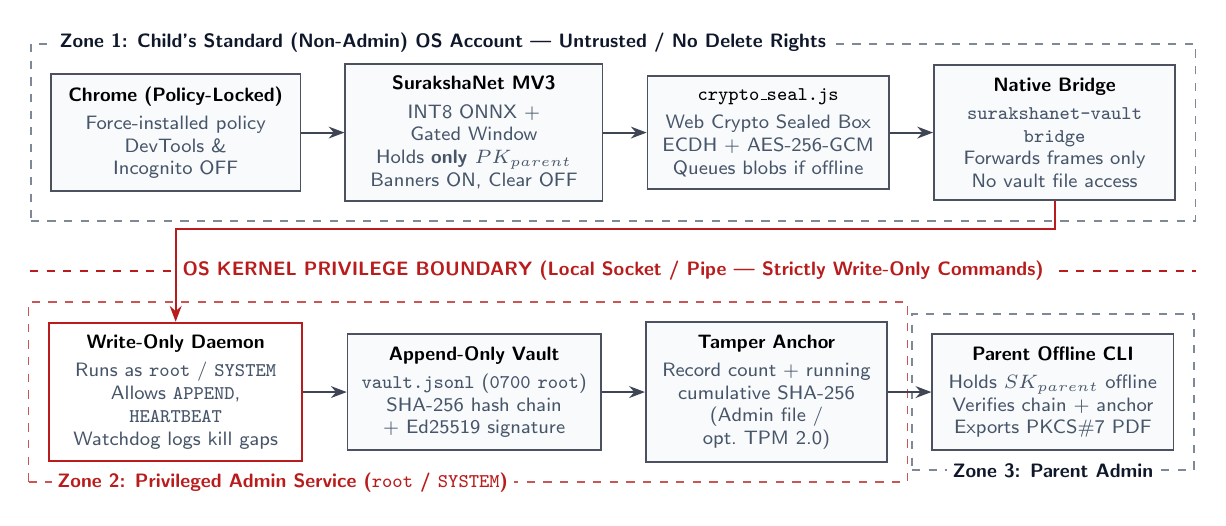
\begin{tikzpicture}
    % Zone 1
    \node[sysbox, text width=2.85cm] (chrome) {\textbf{Chrome (Policy-Locked)}\\[2pt]{\color{slate}Force-installed policy\\DevTools \& Incognito OFF}};
    \node[sysbox, text width=2.95cm, right=0.55cm of chrome] (ext) {\textbf{SurakshaNet MV3}\\[2pt]{\color{slate}INT8 ONNX + Gated Window\\Holds \textbf{only} $PK_{\text{parent}}$\\Banners ON, Clear OFF}};
    \node[sysbox, text width=2.75cm, right=0.55cm of ext] (seal) {\textbf{\texttt{crypto\_seal.js}}\\[2pt]{\color{slate}Web Crypto Sealed Box\\ECDH + AES-256-GCM\\Queues blobs if offline}};
    \node[sysbox, text width=2.75cm, right=0.55cm of seal] (bridge) {\textbf{Native Bridge}\\[2pt]{\color{slate}\texttt{surakshanet-vault bridge}\\Forwards frames only\\No vault file access}};

    \begin{scope}[on background layer]
      \node[syszone, fit=(chrome)(ext)(seal)(bridge),
            label={[fill=white, inner sep=2pt, font=\scriptsize\bfseries, text=ink, anchor=west, xshift=3mm]north west:Zone 1: Child's Standard (Non-Admin) OS Account --- Untrusted / No Delete Rights}] (z1) {};
    \end{scope}

    % Kernel boundary
    \coordinate (bL) at ($(z1.south west)+(0,-0.62cm)$);
    \coordinate (bR) at ($(z1.south east)+(0,-0.62cm)$);
    \draw[accent, thick, dashed] (bL) -- (bR)
      node[midway, fill=white, font=\scriptsize\bfseries, text=accent, inner sep=3pt]
      {OS KERNEL PRIVILEGE BOUNDARY (Local Socket / Pipe --- Strictly Write-Only Commands)};

    % Zone 2 & 3
    \node[sysboxacc, text width=2.9cm, below=1.65cm of chrome] (ipc) {\textbf{Write-Only Daemon}\\[2pt]{\color{slate}Runs as \texttt{root} / \texttt{SYSTEM}\\Allows \texttt{APPEND}, \texttt{HEARTBEAT}\\Watchdog logs kill gaps}};
    \node[sysbox, text width=2.9cm, right=0.55cm of ipc] (chain) {\textbf{Append-Only Vault}\\[2pt]{\color{slate}\texttt{vault.jsonl} (\texttt{0700 root})\\SHA-256 hash chain\\+ Ed25519 signature}};
    \node[sysbox, text width=2.75cm, right=0.55cm of chain] (anchor) {\textbf{Tamper Anchor}\\[2pt]{\color{slate}Record count + running\\cumulative SHA-256\\(Admin file / opt.\ TPM 2.0)}};
    \node[sysbox, text width=2.75cm, right=0.55cm of anchor] (parent) {\textbf{Parent Offline CLI}\\[2pt]{\color{slate}Holds $SK_{\text{parent}}$ offline\\Verifies chain + anchor\\Exports PKCS\#7 PDF}};

    \begin{scope}[on background layer]
      \node[syszone, draw=accent!75, fit=(ipc)(chain)(anchor),
            label={[fill=white, inner sep=2pt, font=\scriptsize\bfseries, text=accent, anchor=west, xshift=3mm]south west:Zone 2: Privileged Admin Service (\texttt{root} / \texttt{SYSTEM})}] (z2) {};
      \node[syszone, fit=(parent),
            label={[fill=white, inner sep=2pt, font=\scriptsize\bfseries, text=ink, anchor=center]south:Zone 3: Parent Admin}] (z3) {};
    \end{scope}

    \draw[sysarr] (chrome) -- (ext);
    \draw[sysarr] (ext) -- (seal);
    \draw[sysarr] (seal) -- (bridge);
    \draw[sysarr, accent] (bridge.south) -- ++(0,-0.36cm) -| (ipc.north);
    \draw[sysarr] (ipc) -- (chain);
    \draw[sysarr] (chain) -- (anchor);
    \draw[sysarr] (anchor) -- (parent);
  \end{tikzpicture}%
  }
  \end{center}
  \vspace{0.15cm}
  {\scriptsize\color{muted}\centering Single cross-platform Go binary (\texttt{surakshanet-vault}) compiled for Linux (\texttt{amd64}), Windows (\texttt{amd64}), and macOS (\texttt{arm64}).\par}
\end{frame}

%==============================================================
% SLIDE 8: PILLAR 1 — OS ADMIN CHROME LOCK (REAL MAC MDM SHOTS)
%==============================================================
\begin{frame}{Pillar 1: Locking Chrome with OS Administrator Policies}
  \begin{columns}[c]
    \begin{column}{0.49\textwidth}
      {\small\bfseries\color{ink} How Extension Removal Is Blocked}
      \vspace{0.1cm}
      \begin{itemize}\footnotesize
        \setlength\itemsep{4.5pt}
        \item Parent runs the installer once as \textbf{OS Admin} (\texttt{install.sh}, \texttt{install.ps1}, or macOS profile).
        \item Writes machine-level \textbf{Chrome Policies}:
          \begin{itemize}\scriptsize
            \setlength\itemsep{2pt}
            \item \texttt{ExtensionInstallForcelist} --- locks extension ON.
            \item \texttt{IncognitoModeAvailability = 1} --- blocks Incognito.
            \item \texttt{DeveloperToolsAvailability = 2} --- blocks DevTools.
          \end{itemize}
        \item \texttt{chrome.storage.managed} pushes \texttt{lockMode: true} and \textbf{only} the parent's public key ($PK_{\text{parent}}$).
        \item Editing or removing the profile requires the \textbf{Admin password}.
      \end{itemize}
    \end{column}
    \begin{column}{0.47\textwidth}
      \centering
      \shot{height=3.0cm}{assets/mac_mdm_password.jpg}\\[5pt]
      \shot{height=2.05cm}{assets/mac_mdm_profile.jpg}\\[3pt]
      {\scriptsize\color{muted} Live macOS test: Admin password lock (top) and installed SurakshaNet Chrome Parent Policy (bottom).}
    \end{column}
  \end{columns}
\end{frame}

%==============================================================
% SLIDE 9: PILLAR 1 LIVE PROOF (chrome://policy + DEVTOOLS BLOCKED)
%==============================================================
\begin{frame}{Pillar 1 Live Verification on macOS Chrome}
  \begin{columns}[c]
    \begin{column}{0.56\textwidth}
      \centering
      \shot{width=\textwidth}{assets/mac_chrome_policy.jpg}\\[4pt]
      {\scriptsize\color{muted} Live \texttt{chrome://policy}: Machine-level Mandatory policies active.}
    \end{column}
    \begin{column}{0.41\textwidth}
      \centering
      \shot{width=\textwidth}{assets/mac_devtools_blocked.jpg}\\[4pt]
      {\scriptsize\color{muted} Live Chrome alert when user attempts to open DevTools.}

      \vspace{0.35cm}
      \raggedright
      {\scriptsize\bfseries\color{ink} Real-World Observation:}\\
      {\scriptsize\color{slate} On non-domain macOS/Windows, Chrome accepts \texttt{DeveloperTools} and \texttt{Incognito} locks locally (\texttt{OK}), while \texttt{ExtensionInstallForcelist} requires a Chrome Web Store ID (an Unlisted listing resolves the warning shown on the left).}
    \end{column}
  \end{columns}
\end{frame}

%==============================================================
% SLIDE 10: PILLAR 2 — ONE-WAY SEALING + REAL MAC LOCKED POPUP
%==============================================================
\begin{frame}{Pillar 2: One-Way Browser Encryption and Locked Popup UI}
  \begin{columns}[c]
    \begin{column}{0.54\textwidth}
      {\small\bfseries\color{ink} Sealed Inside Chrome, Readable Only by Parent}
      \vspace{0.15cm}
      \begin{itemize}\footnotesize
        \setlength\itemsep{6.5pt}
        \item \texttt{extension\_v2/crypto\_seal.js} uses browser built-in \textbf{Web Crypto API} (zero external packages).
        \item For each flagged message, Chrome creates a one-time \textbf{ECDH P-256} keypair, combines it with $PK_{\text{parent}}$ via \textbf{HKDF-SHA256}, and encrypts with \textbf{AES-256-GCM}.
        \item The temporary private key is discarded immediately --- \textbf{not even the extension can read the message back}.
        \item \textbf{WhatsApp warning banners remain live}, while the popup removes plain chat text and the \textit{Clear} button.
        \item If the daemon is momentarily offline, Chrome buffers \textit{only encrypted blobs}.
      \end{itemize}
    \end{column}
    \begin{column}{0.42\textwidth}
      \centering
      \shot{height=5.6cm}{assets/mac_popup_locked.jpg}\\[3pt]
      {\scriptsize\color{muted} Live MacBook Chrome popup: 28 flagged, LOCKED, Chain Seq \#74, zero plaintext.}
    \end{column}
  \end{columns}
\end{frame}

%==============================================================
% SLIDE 11: PILLAR 3 — WRITE-ONLY DAEMON & HASH CHAIN
%==============================================================
\begin{frame}{Pillar 3: Write-Only Admin Daemon and Hash-Chained Log}
  \vspace{0.05cm}
  \begin{center}
  \resizebox{0.99\textwidth}{!}{%
  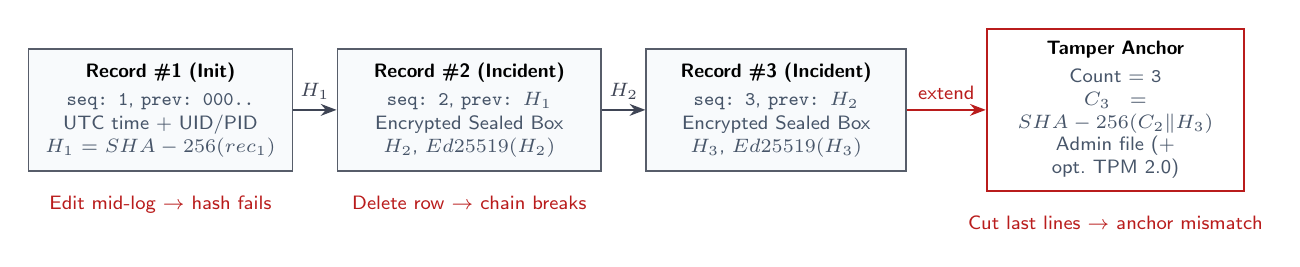
\begin{tikzpicture}
    \node[flowbox, text width=3.0cm] (r1) {\textbf{Record \#1 (Init)}\\[2pt]{\color{slate}\texttt{seq: 1}, \texttt{prev: 000..}\\UTC time + UID/PID\\$H_1 = \text{SHA-256}(\text{rec}_1)$}};
    \node[flowbox, text width=3.0cm, right=0.55cm of r1] (r2) {\textbf{Record \#2 (Incident)}\\[2pt]{\color{slate}\texttt{seq: 2}, \texttt{prev: $H_1$}\\Encrypted Sealed Box\\$H_2$, $\text{Ed25519}(H_2)$}};
    \node[flowbox, text width=2.95cm, right=0.55cm of r2] (r3) {\textbf{Record \#3 (Incident)}\\[2pt]{\color{slate}\texttt{seq: 3}, \texttt{prev: $H_2$}\\Encrypted Sealed Box\\$H_3$, $\text{Ed25519}(H_3)$}};
    \node[sysboxacc, text width=2.95cm, right=1.0cm of r3] (anc) {\textbf{Tamper Anchor}\\[2pt]{\color{slate}Count = \texttt{3}\\$C_3 = \text{SHA-256}(C_2 \Vert H_3)$\\Admin file (+ opt.\ TPM 2.0)}};

    \draw[sysarr] (r1) -- node[above, font=\scriptsize]{$H_1$} (r2);
    \draw[sysarr] (r2) -- node[above, font=\scriptsize]{$H_2$} (r3);
    \draw[sysarr, accent] (r3) -- node[above, font=\scriptsize\color{accent}]{extend} (anc);

    \node[font=\fontsize{6.6}{7.6}\selectfont, text=accent, below=0.18cm of r1] {Edit mid-log $\rightarrow$ hash fails};
    \node[font=\fontsize{6.6}{7.6}\selectfont, text=accent, below=0.18cm of r2] {Delete row $\rightarrow$ chain breaks};
    \node[font=\fontsize{6.6}{7.6}\selectfont, text=accent, below=0.18cm of anc] {Cut last lines $\rightarrow$ anchor mismatch};
  \end{tikzpicture}%
  }
  \end{center}

  \vspace{0.35cm}
  {\color{rulegray}\hrule height 0.5pt}
  \vspace{0.25cm}

  \begin{columns}[T]
    \begin{column}{0.48\textwidth}
      {\footnotesize\bfseries\color{ink} Why Bridge and Daemon Are Separate}\\[4pt]
      \begin{itemize}\scriptsize
        \setlength\itemsep{4pt}
        \item Chrome spawns \texttt{bridge} under the child's account; \texttt{bridge} only relays frames and has no file access.
        \item \texttt{daemon} runs as \texttt{root} / \texttt{SYSTEM} and owns the locked \texttt{0700} / NTFS vault folder.
        \item IPC accepts only \texttt{APPEND\_INCIDENT}, \texttt{HEARTBEAT}, and \texttt{STATUS} --- \textbf{no \texttt{READ} or \texttt{DELETE} command exists}.
      \end{itemize}
    \end{column}
    \begin{column}{0.48\textwidth}
      {\footnotesize\bfseries\color{ink} How Tampering and Kills Are Caught}\\[4pt]
      \begin{itemize}\scriptsize
        \setlength\itemsep{4pt}
        \item \texttt{vault.jsonl} is written via strict \texttt{O\_APPEND} + \texttt{fsync} (plus Linux \texttt{chattr +a} when supported).
        \item Every record carries a SHA-256 link to the previous line and an Ed25519 daemon signature.
        \item A heartbeat watchdog logs \texttt{TAMPER\_HEARTBEAT\_GAP} if anyone stops the extension or kills the bridge.
      \end{itemize}
    \end{column}
  \end{columns}
\end{frame}

%==============================================================
% SLIDE 12: PILLAR 3 LIVE PROOF ON MACBOOK TERMINAL
%==============================================================
\begin{frame}{Pillar 3 Live Proof: Permission Lock and 1-Char Log Tamper}
  \centering
  \shot{height=2.95cm}{assets/mac_term_perm_verify.jpg}\\[2pt]
  {\scriptsize\color{muted} \textbf{Test 1 (Access Lock):} Standard user gets \texttt{Permission denied}; Admin \texttt{verify} confirms \texttt{VERIFIED (INTACT)}.}

  \vspace{0.2cm}

  \shot{height=2.2cm}{assets/mac_term_tamper_log.jpg}\\[2pt]
  {\scriptsize\color{muted} \textbf{Test 2 (1-Char Edit):} Editing 1 char on line 5 via \texttt{sed} triggers \texttt{TAMPERING DETECTED: content hash mismatch}.}
\end{frame}

%==============================================================
% SLIDE 13: PILLAR 4 — OFFLINE PARENT EXPORT & SIGNED PDF
%==============================================================
\begin{frame}{Pillar 4: Offline Parent Audit and Digitally Signed PDF}
  \begin{columns}[c]
    \begin{column}{0.49\textwidth}
      {\small\bfseries\color{ink} Three-Step Offline Parent Review}
      \vspace{0.08cm}
      \begin{enumerate}\footnotesize
        \setlength\itemsep{4.5pt}
        \item \textbf{\texttt{surakshanet-vault verify}}\\
              Reads \texttt{vault.jsonl} directly as Admin and checks every sequence number, SHA-256 link, Ed25519 signature, and anchor match.
        \item \textbf{\texttt{surakshanet-vault export}}\\
              Parent supplies offline \texttt{parent.key.json} (passphrase + \texttt{scrypt}), decrypts all multilingual incidents, and writes a signed PDF.
        \item \textbf{\texttt{surakshanet-vault verify-pdf}}\\
              Any teacher, school, or authority verifies the report using the public certificate \texttt{parent.crt.pem}.
      \end{enumerate}

      \vspace{0.16cm}
      {\color{rulegray}\hrule height 0.5pt}
      \vspace{0.12cm}
      {\scriptsize\color{slate} Uses ISO 32000-1 \textbf{PKCS\#7 / CMS detached signatures} covering the full PDF byte range (\texttt{/ByteRange} from byte 0 to EOF).}
    \end{column}
    \begin{column}{0.47\textwidth}
      \centering
      \shot{width=0.95\textwidth}{assets/signed_pdf_preview.png}\\[4pt]
      {\scriptsize\color{muted} Rendered page of an exported PKCS\#7 signed evidence report.}
    \end{column}
  \end{columns}
\end{frame}

%==============================================================
% SLIDE 14: PILLAR 4 LIVE PROOF ON MACBOOK TERMINAL
%==============================================================
\begin{frame}{Pillar 4 Live Proof: Valid Signature vs.\ 1-Byte PDF Tamper}
  \centering
  \shot{width=0.84\textwidth}{assets/mac_term_pdf_ok.jpg}\\[3pt]
  {\scriptsize\color{muted} \textbf{Original Exported PDF:} \texttt{verify-pdf} confirms valid signer (\texttt{26aeb710ead32b12}) and full \texttt{/ByteRange [0 510 16896 16578]}.}

  \vspace{0.32cm}

  \shot{width=0.84\textwidth}{assets/mac_term_pdf_tamper.jpg}\\[3pt]
  {\scriptsize\color{muted} \textbf{After Flipping 1 Byte (\texttt{dd} at offset 20{,}000):} Verification fails with \texttt{pkcs7: Message digest mismatch}.}

  \vspace{0.22cm}
  {\scriptsize\color{slate} Also verified: IPC \texttt{DELETE\_ALL} is rejected (\texttt{forbidden action}), and cutting the last log line triggers \texttt{TAIL TRUNCATION DETECTED}.}
\end{frame}

%==============================================================
% SLIDE 15: SECURITY SUMMARY & REAL LATENCY BENCHMARKS
%==============================================================
\begin{frame}{Security Comparison and Measured Runtime Overhead}
  \begin{columns}[c]
    \begin{column}{0.46\textwidth}
      {\scriptsize\bfseries\color{ink} ATTACK-BY-ATTACK COMPARISON}\\[6pt]
      \scriptsize
      \renewcommand{\arraystretch}{1.28}
      \begin{tabular}{@{}p{2.05cm} p{1.25cm} >{\raggedright\arraybackslash}p{2.5cm}@{}}
        \toprule
        \textbf{Attack} & \textbf{Before} & \textbf{After (Vault)} \\
        \midrule
        Uninstall ext. & 2 clicks & \textbf{Blocked} (Policy) \\
        Click \textit{Clear} & Wiped & \textbf{Hidden \& blocked} \\
        Read disk logs & Plaintext & \textbf{Denied + Encrypted} \\
        IPC \texttt{DELETE} & N/A & \textbf{Rejected} \\
        Edit / cut log & Silent & \textbf{Caught} (Chain+Anchor) \\
        Edit 1B of PDF & Silent & \textbf{Caught} (PKCS\#7) \\
        \bottomrule
      \end{tabular}

      \vspace{0.35cm}
      {\color{accent}\hrule height 0.8pt}
      \vspace{0.18cm}
      {\scriptsize\color{ink}\textbf{Total capture overhead: 3.60\,ms}} {\scriptsize\color{slate}(0.70\,ms seal + 2.90\,ms daemon save) --- runs only when abuse is flagged, tiny compared to \textbf{28\,ms} AI inference.}
    \end{column}
    \begin{column}{0.51\textwidth}
      \centering
      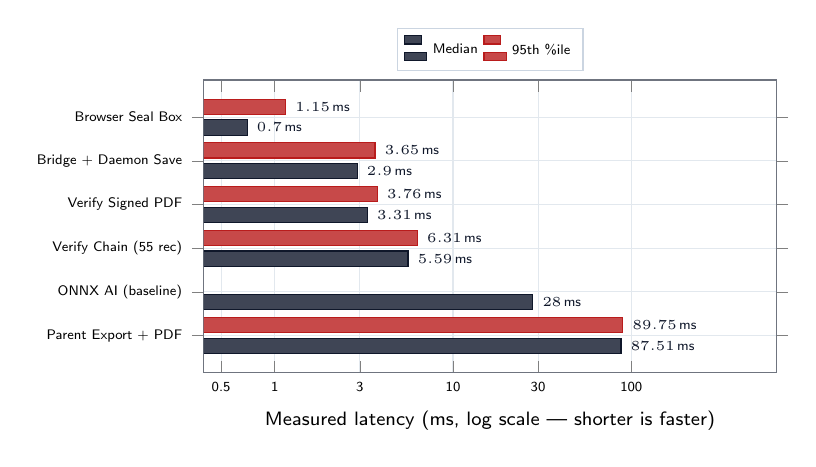
\begin{tikzpicture}
      \begin{axis}[
        xbar,
        width=0.73\textwidth,
        height=5.3cm,
        bar width=5.5pt,
        enlarge y limits=0.17,
        xlabel={\fontsize{6.6}{7.6}\selectfont Measured latency (ms, log scale --- shorter is faster)},
        xmode=log,
        log origin=infty,
        xmin=0.4, xmax=650,
        xtick={0.5, 1, 3, 10, 30, 100},
        xticklabels={0.5, 1, 3, 10, 30, 100},
        tick label style={font=\tiny},
        axis line style={ink!60},
        symbolic y coords={
          {Parent Export + PDF},
          {ONNX AI (baseline)},
          {Verify Chain (55 rec)},
          {Verify Signed PDF},
          {Bridge + Daemon Save},
          {Browser Seal Box}
        },
        ytick=data,
        point meta=rawx,
        nodes near coords={\pgfmathprintnumber[fixed,precision=2]{\pgfplotspointmeta}\,ms},
        nodes near coords style={font=\tiny, anchor=west, color=ink},
        legend columns=2,
        legend style={at={(0.5,1.03)}, anchor=south, font=\tiny,
                      draw=rulegray, fill=white, inner sep=2.5pt},
        grid=major,
        major grid style={rulegray!55},
      ]
        \addplot[fill=ink!80, draw=ink] coordinates {
          (0.70,{Browser Seal Box})
          (2.90,{Bridge + Daemon Save})
          (3.31,{Verify Signed PDF})
          (5.59,{Verify Chain (55 rec)})
          (28.00,{ONNX AI (baseline)})
          (87.51,{Parent Export + PDF})
        };
        \addplot[fill=accent!80, draw=accent] coordinates {
          (1.15,{Browser Seal Box})
          (3.65,{Bridge + Daemon Save})
          (3.76,{Verify Signed PDF})
          (6.31,{Verify Chain (55 rec)})
          (89.75,{Parent Export + PDF})
        };
        \legend{Median, 95th \%ile}
      \end{axis}
      \end{tikzpicture}
    \end{column}
  \end{columns}
\end{frame}

%==============================================================
% SLIDE 16: HONEST LIMITATIONS & FUTURE WORK
%==============================================================
\begin{frame}{Honest Limitations and Future Work}
  \vspace{0.15cm}
  \begin{columns}[T]
    \begin{column}{0.47\textwidth}
      {\fontsize{16}{18}\selectfont\bfseries\color{rulegray} 01}\quad{\small\bfseries\color{ink} Full Disk Wipe or Admin Theft}\\[4pt]
      {\footnotesize\color{slate} A purely local vault cannot survive a hard-drive format or an attacker who knows the OS Admin password. \textit{Next:} optional zero-knowledge upload of already-encrypted blobs to write-once backup storage.}

      \vspace{0.55cm}

      {\fontsize{16}{18}\selectfont\bfseries\color{rulegray} 02}\quad{\small\bfseries\color{ink} Consumer macOS / Windows Policy}\\[4pt]
      {\footnotesize\color{slate} As shown on Slide~9, Chrome on non-domain macOS/Windows restricts \texttt{ExtensionInstallForcelist} to Chrome Web Store IDs. Publishing an Unlisted store package solves this cleanly.}
    \end{column}
    \begin{column}{0.47\textwidth}
      {\fontsize{16}{18}\selectfont\bfseries\color{rulegray} 03}\quad{\small\bfseries\color{ink} Synthetic Five-Class Data}\\[4pt]
      {\footnotesize\color{slate} Our 105{,}000-thread five-class dataset was generated by Qwen3-32B with rule checks. Zero-shot tests on real data (CAD, ConvAbuse, PRISM) gave 0.47--0.74 AUROC, so real human-labelled chats should be mixed in before deployment.}

      \vspace{0.55cm}

      {\fontsize{16}{18}\selectfont\bfseries\color{rulegray} 04}\quad{\small\bfseries\color{ink} Hardware \& External Time Proofs}\\[4pt]
      {\footnotesize\color{slate} Our daemon already supports optional TPM~2.0 anchoring; future work adds RFC~3161 trusted timestamps and network-level TLS provenance.}
    \end{column}
  \end{columns}
\end{frame}

%==============================================================
% SLIDE 17: CONCLUSION & QUESTIONS
%==============================================================
\begin{frame}[plain]
  \begin{tikzpicture}[remember picture,overlay]
    \fill[ink] (current page.north west) rectangle (current page.south east);
    \fill[accent] (current page.north west) rectangle ([xshift=0.28cm]current page.south west);
  \end{tikzpicture}

  \vspace*{0.9cm}
  {\fontsize{9}{11}\selectfont\bfseries\color{accent} CONCLUSION}\\[0.25cm]
  {\fontsize{24}{28}\selectfont\bfseries\color{white} Practical, Privacy-First Safety\\for Families and Evidence}\\[0.55cm]

  \begin{columns}[T]
    \begin{column}{0.24\textwidth}
      {\Large\bfseries\color{white} 100\%}\\[2pt]
      {\scriptsize\color{white!70} Offline privacy\\(zero cloud plaintext)}
    \end{column}
    \begin{column}{0.24\textwidth}
      {\Large\bfseries\color{white} 28\,ms}\\[2pt]
      {\scriptsize\color{white!70} On-device Hinglish\\abuse detection}
    \end{column}
    \begin{column}{0.24\textwidth}
      {\Large\bfseries\color{white} 3.6\,ms}\\[2pt]
      {\scriptsize\color{white!70} Tamper-evident vault\\capture overhead}
    \end{column}
    \begin{column}{0.24\textwidth}
      {\Large\bfseries\color{white} 4 Pillars}\\[2pt]
      {\scriptsize\color{white!70} Admin lock, sealing,\\chain, signed PDF}
    \end{column}
  \end{columns}

  \vspace{0.75cm}
  {\color{white!25}\hrule height 0.5pt}
  \vspace{0.45cm}

  {\Large\bfseries\color{white} Thank You --- Questions?}\\[0.15cm]
  {\footnotesize\color{white!75} Source Code, Extension, Go Vault Binary \& Technical Report: \;\texttt{github.com/PrathamGarg1/surakshanet}}
\end{frame}

\end{document}
